
Comme on vient de voir dans les chapitres précédents, de nombreux phénomènes dans des contextes très variés peuvent être représentés par des graphes. Citons en particuliers les réseaux sociaux qui nous attirent vu leur importance et leur fort impact sur la vie réelle. En effet, trois quarts des personnes connectées à Internet utilisent les réseaux sociaux. Ils rassemblent aujourd'hui 3,169 milliards d'utilisateurs actifs, voir 40\% de la population sur terre, avec 11 personnes s'inscrivant chaque seconde sur Facebook, Twitter et autres
\footnote{https://bfmbusiness.bfmtv.com/hightech/la-moitie-de-la-population-mondiale-est-connectee-a-internet-1361933.html}. De ce fait, deux constats s'imposent: le premier est l'incapacité des graphes statiques à décrire certaines situations de la vie réelle et leur évolution dans le temps, le deuxième est la montée en flèche de la quantité et l'hétérogénéité des informations modélisées par ces réseaux et qui rendent presque impossible tout traitement. D'où le besoin croissant de méthodes de compression de graphes dynamiques. 

Nous nous sommes aussi intéressées dans ce travail à un autre enjeu important qui est la recherche de motifs et particulièrement les cliques et les noyaux bipartis qui sont fréquents dans les réseaux faisant abstraction à des situations réelles importantes dans le processus de prise de décision. Nous citons par exemple, les attaquants de réseaux de botnet formant un noyau biparti avec leurs victimes pendant la durée d'une attaque, les membres de la famille se liant comme une clique au cours d'une période difficile, ou les collaborations de recherche s'étant créées et qui disparaissent au cours des années.

%Quoiqu'il existe de nombreuses techniques de compression efficaces adaptées au contexte statique, rares sont ceux qui proposent une contrepartie dynamique, ce qui nous amène à s'intéresser particulièrement à ce type de graphes toujours en cours d'évolution. 

Nous allons dans cette partie proposer une nouvelle méthode \gls{ddsm} basée sur deux approches existantes. Notre but principal est de développer une technique de compression compétitive pour les graphes des réseaux d'interactions dans un contexte dynamique en se basant sur l'extraction de motifs pour filtrer les informations les plus importantes et les arbres $k^2$-trees pour aboutir à une compression sans perte. Pour accomplir ce travail nous nous sommes appuyées sur les deux techniques suivantes:
\begin{itemize}
\item Exploiter la structure de données proposée dans \gls{dsm} \citep{hernandez2014compressed} qui permet de représenter les sous-graphes denses comme les cliques, les quasi-cliques, noyaux bipartis de manière concise. Nous avons opté pour cette structure car  elle donne de bons résultats en matière d'espace et de temps de requêtes.  
\item Adopter les signatures temporelles utilisées dans TimeCrunch \citep{shah2015timecrunch} pour décrire le comportement des sous-graphes dans le temps. Nous avons utilisé ces signatures car elles englobent tous les types de comportements temporels d'un motif dans un graphe dynamique.
\end{itemize}	
%Nous allons dans cette partie présenter notre méthode théoriquement : principe général, structure utilisée et un pseudo code.	
		
		\subsection{Formulation du problème}
		Dans cette section, nous allons définir le problème de base auquel notre méthode convient tout en définissant le cadre dans lequel elle peut être appliquée. 
		
		Nous considérons les graphes orientés dynamiques $\displaystyle{G=\bigcup_{t_{i}}G_{t_{i}}(V,E_{t_{i}})}\ \ 1 \preceq i \preceq t$ où $G_{t_{i}}$ = G à l'instant $t_{i}$ et un ensemble de signatures temporelles. En d'autre termes, nous considérons des captures du graphe à des instants différents $t_{i}$ et un ensemble de descripteurs de comportement temporel des sous-graphes des différents $G_{t_{i}}$. Le problème peut ainsi être formulé:
		
			\textit{\textbf{Problème:}
		Trouver, à partir d'un graphe dynamique G et un lexique de signatures temporelles, la plus petite description du graphe initial en termes de ses sous structures les plus denses et leur comportement temporel, en offrant la possibilité de manipuler le graphe, d'extraire les voisins directs d'un nœud à un instant donné et d'extraire les sous-graphes au besoin. }

		\subsection{Principe général}
			Notre méthode s'intitule DDSM pour \textit{Dynamic Dense Substructure Mining}. Elle représente une généralisation du travail de Hernandez et Navarro \citep{hernandez2014compressed} pour le cas des graphes dynamiques qui sont de nos jours omniprésents.
			
			%Pour mieux expliquer notre méthode nous allons tout d'abord commencer par décrire les structures que nous allons utiliser. Nous enchainons par la suite  avec le pseudo algorithme détaillant les étapes essentielles de notre méthode et nous conclurons en expliquant comment les algorithmes proposés dans \citep{hernandez2014compressed} de manipulation des graphes peuvent être généralisés dans notre cas.
			%\subsection{Description conceptuelle}
			
			La codification du graphe en sortie doit respecter les contraintes du problème tout en réduisant un maximum d'espace mémoire. Pour cela, nous proposons d'étendre la codification proposée dans \citep{hernandez2014compressed} pour le cas des graphes dynamiques en rajoutant une information temporelle. Une fois les sous-structures identifiées, Hernandez et al. \citep{hernandez2014compressed} proposent de représenter chacune d'elles avec trois composantes: la première contenant les sommets ayant uniquement des arêtes sortantes, la deuxième contenant les sommets ayant des arêtes entrantes et sortantes et la troisième contenant les sommets ayant uniquement des arêtes entrantes. Pour pouvoir identifier les différentes composantes, ils associent un vecteur binaire à cette représentation marquant par un 1 le début de chacune des trois composantes (voir figure \ref{SDM}). Notre première contribution consiste en l'extension de cette structure. En effet, nous suggérons de représenter chaque sous structure avec non pas trois composantes mais quarte composantes. Les trois premières étant les même que dans \citep{hernandez2014compressed}, la quatrième représente l'information temporelle. Cette dernière peut avoir cinq formats (voir section \ref{par:TimeCrunch}) dont nous résumons la représentation proposée pour chacune dans le tableau \ref{tab:signtmp}.
			
			\begin{table}[h]
			
			\begin{center}
			\begin{tabular}{|r|l|}
			\hline Signature temporelle & Représentation	
			\\\hline constante & 0	
			
			\\\hline OneShot & 1 $t_{1}$	
			
			\\\hline ranged & 2	$t_{1}\ t_{2}$	
			
			\\\hline periodic & 3  $T$	
			
			\\\hline flikering & 4 $t_{1}\ t_{2}\ ...\ t_{n}$	
			
			\\\hline			
			\end{tabular}
			\end{center}
			
			 \caption{\small {Les types de signatures temporelles et leurs représentations, $t_{i}$	 représentent les timestamps et T représente la période.}}
				\label{tab:signtmp}			
			\end{table}
			
			Nous représentons G donc comme un ensemble de sous-graphes temporels denses. Cependant, pour obtenir une compression sans perte, nous devons aussi garder l'erreur modélisant l'ensemble d'arêtes restantes dans chaque $G_{t_{i}}$. Nous proposons pour cela d'utiliser une des structures dynamiques des k2-trees qui nous permettra de garder trace de cette dernière dans un format compacte. Nous ferons appel à cette étape au moteur $k^2$-GraCE.
			
			%\subsection{Notre méthode : DDSM}
			 Nous visons à travers la méthode que nous proposons d'exprimer le graphe en entrée avec ses sous-structures les plus denses et leur comportement temporel réduisant ainsi sa taille et offrant la possibilité d'effectuer les traitements dans un temps meilleur. Nous avons structuré notre algorithme sous forme de trois (03) étapes essentielles, chacune servant d'entrée pour l'étape suivante.
			 
			 En premier lieu, nous appliquons la découverte des sous-graphes les plus denses. Pour effectuer cela de manière efficace, nous suggérons d'utiliser la technique du MinHashing du moteur P-GraCE parallèlement sur chaque capture $G_{t_{i}}$ de G. 
			 
			 
			 Dans une deuxième phase, nous effectuons une comparaison entre les sous-structures. Nous utilisons pour cela le principe du MinHashing encore une fois pour grouper les sous-structures de différents timestamps ayant un nombre élevé de nœuds en commun. Ayant associé à chaque sous-structure ses différents timestamps, ces derniers seront à leur tour compressés en utilisant les descripteurs de comportement temporel précédemment décrits. L'algorithme \ref{alg:getTemporalSignature} représente les étapes de compression de l'ensemble des timestamps d'une structure.\\
			 
			 
			 	\begin{algorithm}[H]
					
					\caption{getTemporalSignature}
					\label{alg:getTemporalSignature}
					\textbf{Entrée :}
						\begin{itemize}[label=$\bullet$]
							\item timeseries[] : un tableau de timestamps
							\item size : la taille du tableau timeseries
						\end{itemize}
					\textbf{Sortie :} la signature temporelle\\							\noindent\rule{\textwidth}{1pt}
						
						
				\begin{algorithmic} [1]
					
					\IF{|timeseries| = T} 
						\STATE return 'c' 	\COMMENT{Constante}
					\ELSE 
						\IF {|timeseries| = 1} 
							\STATE return 'o' \COMMENT{OneShot}
						\ELSE
							\IF{$t_{i+1} -t_i$ =1 $\forall t_i \in $ timeseries}
								\STATE return 'r' : timeseries[0] :timeseries[size-1] \COMMENT{Ranged}
							\ELSE
								\IF {{$t_{i+1} -t_i$ = Constante $\forall t_i \in $ timeseries}}
									\STATE retourner 'p' : timeseries[1] - timeseries [0] \COMMENT{periodic}
								\ELSE
									\STATE return 'f':timeseries[0]:...:timeseries[size-1] \COMMENT{flickering}
								\ENDIF							
							\ENDIF
						\ENDIF
					\ENDIF
					
				\end{algorithmic}
			\end{algorithm}
			 
			 
			 \vskip 0.1in
			 
			 Une dernière phase consiste en la codification du graphe en utilisant le codage proposé pour chaque sous-structure de la phase (02). Nous concaténons par la suite ces représentations pour obtenir une seule représentation concise du graphe initial en terme de ses structures les plus denses. Nous schématisons ces différentes étapes dans la figure \ref{ddsmScheme}.
			 
			 

			  
			L'algorithme \ref{alg:DDSM} représente l'algorithme de compression globale.
			\begin{algorithm}
					
					\caption{DDSM}
					\label{alg:DDSM}
					%\label{Pseudo Algorithme de la méthode proposée (DDSM)}
				\begin{algorithmic} [1]
					\STATE \textbf{Génération des sous structures candidates: }Génération de sous-graphes, principalement les bicliques et les cliques.
					
					\STATE  \textbf{Étiquetage de sous-structures: }Associer chaque sous-structure à une signature temporelle décrivant son comportement.
					
					\STATE \textbf{Codification du graphe compressé: }Codifier les sous-structures étiquetées de l'étape (02) en utilisant les structures de la section précédente.
				\end{algorithmic}
			\end{algorithm}
			
			
		Pour les algorithmes de parcours et d'extraction de voisins, tous les algorithmes proposés dans \citep{hernandez2014compressed} peuvent être généralisés sur notre structure. En effet, le seul changement consiste en la  prise en compte de l'information temporelle dans l'incrémentation des indices de parcours. De ce fait, nous pensons que notre méthode peut offrir un très bon compromis entre l'espace mémoire et le temps d'accès des traitements dans le cas des graphes dynamiques. 
		
		\begin{figure}[H]
\centering
	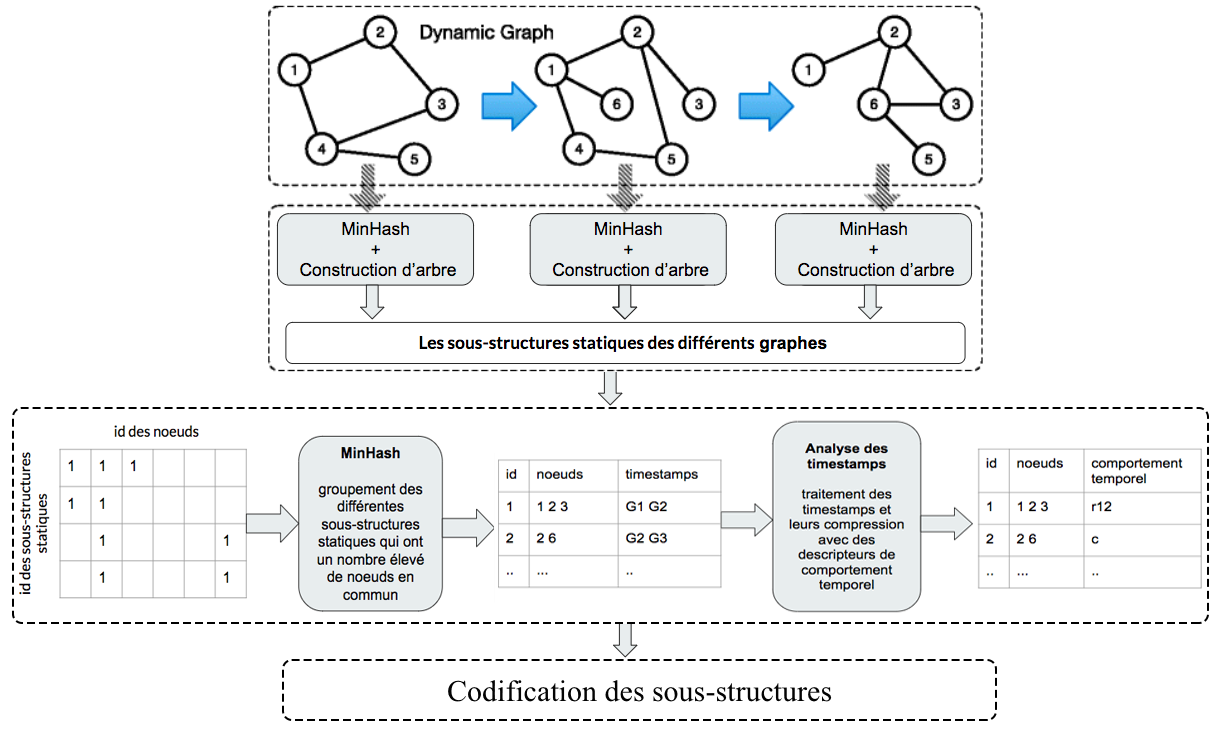
\includegraphics[scale=0.4]{./ressources/image/ddsm_scheme.png}
	\caption[Les différentes phases de DDSM]{Les différentes phases de DDSM}
	\label{ddsmScheme}
\end{figure}
			
		%\subsubsection{Conclusion}
	%Dans ce chapitre, nous avons abordé le problème de compression des graphes dynamiques par extraction de motifs. Nous avons formalisé le problème de compression d'un graphe dynamique en se basant sur les sous-graphes denses temporelles qui le composent. Pour faire face à ce problème nous avons présenté une nouvelle méthode hybride intitulée DDSM, elle combine deux méthodes de la littérature que nous avons jugé efficaces. Notre prochain but est de tester cette méthode en la comparant avec les méthodes existantes.   

	